\newcommand{\EART}{$\mathbb{E}_{ART}$}
\newcommand{\ED}{$\mathbb{E}_d$}

%% START FAVITES CHAPTER
\chapter{\favitestitle}
\label{chap:favites}
\clearpage

\textit{Motivation} --- The ability to simulate epidemics as a function of model parameters allows insights that are unobtainable from real datasets. Further, reconstructing transmission networks for fast-evolving viruses like \gls{HIV} may have the potential to greatly enhance epidemic intervention, but transmission network reconstruction methods have been inadequately studied, largely because it is difficult to obtain ``truth'' sets on which to test them and properly measure their performance.

\textit{Results} --- We introduce FAVITES, a robust framework for simulating realistic datasets for epidemics that are caused by fast-evolving pathogens like \gls{HIV}. FAVITES creates a generative model to produce contact networks, transmission networks, phylogenetic trees, and sequence datasets, and to add error to the data. FAVITES is designed to be extensible by dividing the generative model into modules, each of which is expressed as a fixed \gls{API} that can be implemented using various models. We use FAVITES to simulate \gls{HIV} datasets and study the realism of the simulated datasets. We then use the simulated data to study the impact of the increased treatment efforts on epidemiological outcomes. We also study two transmission network reconstruction methods and their effectiveness in detecting fast-growing clusters.

\textit{Availability and implementation} --- FAVITES is available at \url{https://github.com/niemasd/FAVITES}, and a Docker image  can be found on DockerHub (\url{https://hub.docker.com/r/niemasd/favites}).

\section{Introduction}
The spread of many infectious diseases is driven by social and sexual networks~\cite{Kelly1991}, and reconstructing their transmission histories from molecular data may be able to enhance intervention. For example, network-based statistics for measuring the effects of \gls{ART} in \gls{HIV} can yield increased statistical power~\cite{Wertheim2011}; the analysis of the growth of \gls{HIV} infection clusters can yield actionable epidemiological information for disease control~\cite{Lewis2008}; transmission-aware models can be used to infer \gls{HIV} evolutionary rates~\cite{Vrancken2014}.

A series of events in which an infected individual infects another individual can be shown as a \textit{transmission network}, which itself is a subset of a \textit{contact network}, a graph in which nodes represent individuals and edges represent contacts (e.g. sexual) between pairs of individuals. If the pathogens of the infected individuals are sequenced, which is the standard of \gls{HIV} care in many developed countries, one can attempt to reconstruct the transmission network (or its main features) using molecular data. Some viruses, such as HIV, evolve quickly, and the phylogenetic relationships between viruses are reflective of transmission histories~\cite{Leitner1996}, albeit imperfectly~\cite{Ypma2013,Romero-Severson2014,Leitner2018}.

Recently, multiple methods have been developed to infer properties of transmission networks from molecular data~\cite{Prosperi2011,Ragonnet-Cronin2013,Pond2018}. Efforts have been made to characterize and understand the promise and limitations of these methods: it is suggested that, when combined with clinical and epidemiological data, these methods can provide critical information about drug resistance, associations between sociodemographic characteristics, viral spread within populations, and the time scales over which viral epidemics occur~\cite{Grabowski2014}. More recently, these methods have become widely used at both local~\cite{Campbell2017} and global scale~\cite{Wertheim2014}. Nevertheless, several questions remain to be fully answered regarding the performance of these methods.  It is not always clear which method/setting combination performs best for a specific downstream use-case or for specific epidemiological conditions.  More broadly, the effectiveness of these methods in helping achieve public health goals is the subject of ongoing clinical and theoretical research.

Accuracy of transmission networks is difficult to assess because the true order of transmissions is not known. Moreover, predicting the impact of parameters of interest (e.g. rate of treatment) on the epidemiological outcomes is difficult. In simulations, in contrast, the ground truth is known and parameters can be easily controlled. The simulation of transmission networks needs to combine models of social network, transmission, evolution, and ideally sampling biases and errors~\cite{Villandre2016}.

We introduce FAVITES (FrAmework for VIral Transmission and Evolution Simulation), which can simulate numerous models of contact networks, viral transmission, phylogenetic and sequence evolution, data (sub)sampling, and real-world data perturbations, and which was built to be flexible such that users can seamlessly plug in statistical models at every step of the simulation process. Previous attempts to create an epidemic simulation tool include epinet~\cite{Groendyke2012}, TreeSim~\cite{Stadler2013}, outbreaker~\cite{Jombart2014}, seedy~\cite{Worby2015}, and PANGEA.HIV.sim~\cite{Ratmann2017}. A detailed comparison of FAVITES with these tools can be found in Table~\ref{tab:favites-comparison}. One key distinction is that FAVITES simulates the full end-to-end epidemic dataset (social contact network, transmission history, incomplete sampling, viral phylogeny, error-free sequences, and real-world sequencing imperfections), whereas each existing tool simulates only a subset of these steps. Another key distinction is that FAVITES allows the user to choose among several models at each step of the simulation, whereas the existing tools are restricted to specific models. After describing the FAVITES framework,  we compare its output to real data on a series of experiments, study the properties of \gls{HIV} epidemics as functions of various model and parameter choices, and finally perform simulation experiments to study two transmission network reconstruction methods.

\section{Materials and Methods}
\subsection{FAVITES simulation process}
\label{sec:favites-process}
FAVITES provides a workflow for the simulation of viral transmission networks, phylogenetic trees, and sequence data (Fig.~\ref{fig:favites-workflow}). It breaks the simulation process into a series of interactions between abstract modules, and users can select the module implementations appropriate to their specific context. In the statistical sense, the end-to-end process creates a complex composite generative model, each module is a template for a sub-model of a larger model, and different implementations of each module correspond to different statistical sub-models. Thus, the FAVITES workflow does not explicitly make model choices: each module \textit{implementation} makes those choices. The model for a FAVITES execution is defined by the set of module implementations chosen by the user.

\begin{figure}[h] 
\centering
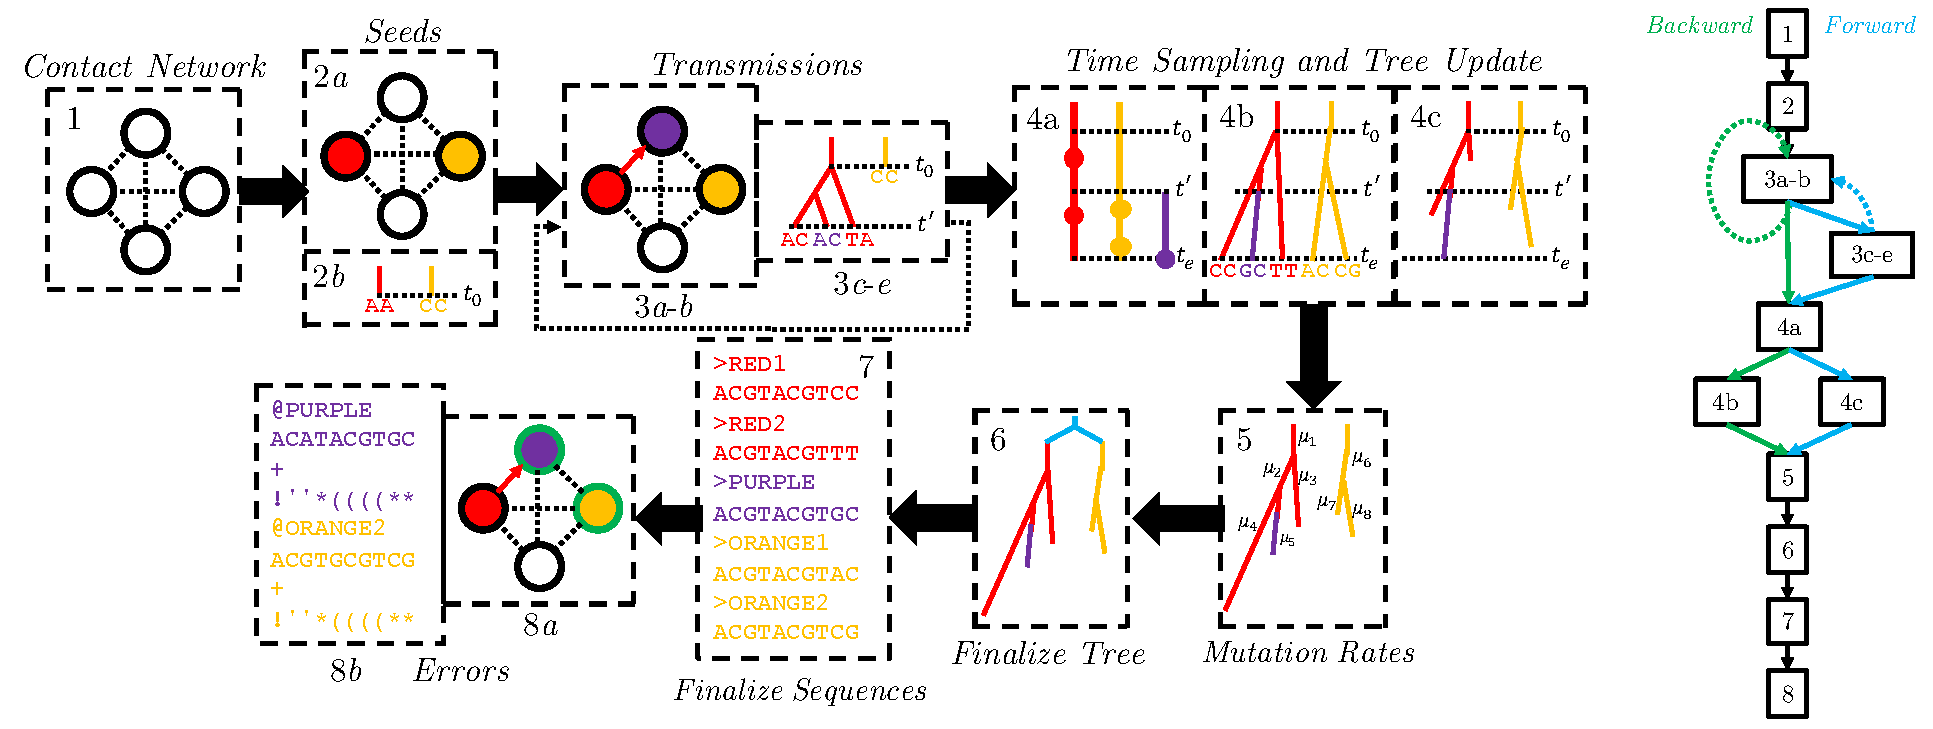
\includegraphics[width=\textwidth]{figs/favites-workflow}
\caption[FAVITES Workflow]
{FAVITES workflow. (1)~The contact network is generated (nodes: individuals; edges: contacts). (2)~\textit{Seed} individuals who are infected at time 0 are selected (2a), and a viral sequence is chosen for each (2b). (3)~The epidemic yields a series of transmission events in which the time of the next transmission is chosen (3a), the source and target individuals are chosen (3b), the viral phylogeny in the source node is evolved to the transmission time (3c), viral sequences in the source node are evolved to the transmission time (3d), and a viral lineage is chosen to be transmitted from source to destination (3e). Step (3) repeats until the end criterion is met.  Step 3c--e are optional, as tree and sequence generation can be delayed to later steps. (4)~Infected individuals are sampled such that viral sequencing times are chosen for each infected individual (4a), viral phylogenies (one per seed) are evolved to the end time of the simulation (4b), and viral phylogenies (one per seed) are pruned to reflect the viral sequencing times selected (4c). (5)~Mutation rates are introduced along the branches of the viral phylogenies  and the tree is scaled to the unit of expected mutations. (6)~ The seed trees are merged using a seed tree (cyan). (7)~Viral sequences obtained from each infected individual are finalized. (8)~Real-world errors are introduced on the error-free data, such as subsampling of the sequenced individuals (marked as green) (8a) and the introduction of sequencing errors (8b). The workflows of a typical forward (blue) and backward (green) simulation are shown as well.}
\label{fig:favites-workflow}
\end{figure}

FAVITES defines \glspl{API} for each module and lets implementation decide how to achieve the goal of the module. The \glspl{API} allow various forms of interaction between modules, which enable sub-models that are described as conditional distributions (via dependence on preceding steps) or as joint distributions (via joint implementation). Module implementations can simply wrap around existing tools, allowing for significant code reuse. The available implementations for each step are continuously updated; the full documentation of these implementations can be found online.

Simulations start at time zero and continue until a user-specified stopping criterion is met. Error-free and error-prone transmission networks, phylogenetic trees, and sequences are output at the end. FAVITES has eight steps (Fig.~\ref{fig:favites-workflow}) detailed below. Depending on the specific implementations, some of the steps may not be needed (we mark these with an asterisk), especially when the phylogeny is simulated backward in time. Also note that steps and modules are not the same; a module may be used in several steps and a step may require multiple modules.

\paragraph{Step 1: Contact Network.} The \textit{ContactNetworkGenerator} module generates a contact network; vertices represent individuals, and edges represent contacts between them that can lead to disease transmission (e.g. sexual). Graphs can be created stochastically using existing models~\cite{Karonski1982}, including those that capture properties of real social networks~\cite{Watts1998,Barabasi1999,Newman2002} and those that include communities~\cite{Watts1999,Fortunato2010}. For example, the \gls{ER} model~\cite{Erdos1960} generates graphs with randomly-placed edges, the Random Partition model~\cite{Fortunato2010} generates communities, the \gls{BA} model~\cite{Barabasi1999} generates scale-free networks whose degree distributions follow power-law (suitable for social and sexual contact networks), the Caveman model~\cite{Watts1999} and its variations~\cite{Fortunato2010} generate small-world networks, the \gls{WS} model~\cite{Watts1998} generates small-world networks with short average path lengths, and Complete graphs connect all pairs of individuals (suitable for some communicable diseases). We currently have many models implemented by wrapping around the NetworkX package~\cite{Hagberg2008}. In addition, a user-specified network can be used.

\paragraph{Step 2: Seeds.} The transmission network is initialized in two steps. $a)$ The \textit{SeedSelection} module chooses the ``seed'' nodes: individuals who are infected at time zero of the simulation. $b^*)$ For each selected seed node, the \textit{SeedSequence} module can generate an initial viral sequence.

Seed selection has many implemented models, including uniform random selection, degree-weighted random selection, and models that place seeds in close proximity. Seed sequences can be user-specified or randomly sampled from probabilistic distributions. To enable seed sequences that emulate the virus of interest, we implement a model that uses HMMER~\cite{Eddy1998} to sample each seed sequence from a profile \gls{HMM} specific to the virus of interest. Profile \glspl{HMM} are appropriate for sampling random sequences that are intended to resemble real sequences because they define a probabilistic distribution over the space of sequences, they can be flexible to insertions and deletions, and they can be sampled in a computationally efficient manner. We provide a set of such prebuilt profile \glspl{HMM} constructed from \glspl{MSA} of viral sequences.

When multiple seeds are chosen, we need to model their phylogenetic relationship as well. Thus, we also have a model that samples a \textit{single} sequence from a viral profile HMM using HMMER, simulates a \textit{seed tree} with a single leaf per seed individual (e.g. using Kingman coalescent or birth-death models using DendroPy~\cite{Sukumaran2010}), and then evolves the viral sequence down the tree to generate seed sequences using Seq-Gen~\cite{Rambaut1997}.

\paragraph{Step 3: Transmissions.} An iterative series of transmission events occurs under a transmission model until the \textit{EndCriteria} module triggers termination (e.g. after a user-specified time or a user-specified number of transmission events). Each transmission event has five components.

$a)$ The \textit{TransmissionTimeSample} module chooses the time at which the next transmission event will occur and advances the \textit{current} time accordingly, and $b)$ the \textit{TransmissionNodeSample} module chooses a source node and target node to be involved in the next transmission event. These two modules are often jointly implemented. Some of the current implementations use simple models such as drawing transmission times from an exponential distribution and selecting nodes uniformly at random. Others are more realistic and use Markov processes in which individuals start in some state (e.g. Susceptible) and transition between states of the model (e.g. Infected) over time. These Markov models are defined by two sets of transition rates: \textit{nodal} and \textit{edge-based}. Nodal transition rates are rates that are independent of interactions with neighbors (e.g. the transition rate from Infected to Recovered), whereas edge-based transition rates are the rate of transitioning from one state to another given that a single neighbor is in a given state (e.g. the transition rate from Susceptible to Infected given that a neighbor is Infected). The rate at which a specific node $u$ transitions from state $a$ to state $b$ is the nodal transition rate from $a$ to $b$ plus the sum of the edge-based transition rate from $a$ to $b$ given neighbor $v$'s state for all neighbors $v$. We use GEMF~\cite{Sahneh2017} to implement many compartmental epidemiological models in this manner, including sophisticated \gls{HIV} models like the Granich \textit{et al}. (2009) model~\cite{Granich2009} and the HPTN 071 (PopART) model~\cite{Cori2014}.

$c^*)$ The \textit{NodeEvolution} module evolves viral phylogenetic trees of the source node to the current time using stochastic models of tree evolution ~\cite{Hartmann2010}. We use DendroPy~\cite{Sukumaran2010} for birth-death  and use our own implementation of dual-birth~\cite{Moshiri2017} and Yule.

$d^*)$ If models of the tree evolution or transmission models are dependent on sequences, the \textit{SequenceEvolution} module is invoked here to evolve all viral sequences in the source node to the current time. Otherwise, sequence evolution is delayed until Step 7 (we assume this scenario).

$e^*)$ The \textit{SourceSample} module chooses the viral lineage(s) in the source node to be transmitted.

\paragraph{Step 4: Time Sampling and Tree Update.} The patient sampling (i.e., sequencing) events are determined and phylogenetic trees are updated accordingly. Three sub-steps are involved.

$a)$ For each individual, the \textit{NumTimeSample} module chooses the number of sequencing times (e.g. a fixed number or a number sampled from a Poisson distribution), the \textit{TimeSample} module chooses the corresponding sequencing time(s) (e.g. by draws from uniform or truncated Gaussian or Exponential distributions, or by sampling right before the first transition of a person to a treated state), and the \textit{NumBranchSample} module chooses how many viral lineages will be sampled at each sequencing time (e.g. single). A given individual may not be sampled at all, thus simulating incomplete epidemiological sampling efforts.

$b^*/c^*)$ The \textit{NodeEvolution} module is called to simulate the phylogenetic trees \textit{given sampling times}. 
This step can be used \textit{instead of} Step 3c to evolve only lineages that are sampled, thereby reducing computational overhead.
If the tree is simulated in Step 3c, it will be pruned here to only include lineages that are sampled.

\paragraph{Step 5: Mutation Rates.} To generate sequences, rates of evolution must be assumed and in this step, the \textit{TreeUnit} module determines such rates. For example, it may use constant rates or may draw from a distribution (e.g. Gamma). Applying rates on the tree from Step 4 yields a tree with branch lengths in units of per-site expected number of mutations.

\paragraph{Step 6$^*$: Finalize Tree.} We now have a single tree per seed. Some implementations of \textit{SeedSequence} also simulate a tree connecting seeds, so the roots of per-seed trees have a phylogenetic relationship. In this case,  this step merges all phylogenetic trees into a single global tree by placing each individual tree's root at its corresponding leaf in the seed tree (Fig.~\ref{fig:favites-workflow}).

\paragraph{Step 7: Finalize Sequences.} The \textit{SequenceEvolution} module is called to simulate sequences on the final tree(s). Commonly-used models of DNA evolution including \gls{GTR} model~\cite{Tavare1986}, and its reductions such as Jukes and Cantor~(1969)~\cite{Jukes1969}, Kimura~(1980)~\cite{Kimura1980}, Felsenstein~(1981)~\cite{Felsenstein1981}, and Tamura and Nei~(1993)~\cite{Tamura1993}, are currently available as implementations of \textit{SequenceEvolution}. FAVITES also includes the \gls{GTR}+$\Gamma$ model, which incorporates rates-across-sites variation~\cite{Yang1994}. It also includes multiple codon-aware extensions of the \gls{GTR} model, such as mechanistic~\cite{Zaheri2014} and empirical~\cite{Kosiol2007} codon models. These modules internally use Seq-Gen~\cite{Rambaut1997} and Pyvolve~\cite{Spielman2015}.

\paragraph{Step 8: Errors.} Error-free data are now at hand. Noise is introduced onto the complete error-free data in two ways.

$a^*)$ The \textit{NodeAvailability} module further subsamples the individuals to simulate lack of accessibility to certain datasets. Note that whether or not an individual is sampled is a function of two different modules: \textit{NodeAvailability} and \textit{NumTimeSample} (if \textit{NumTimeSample} returned 0, the individual is not sampled). Conceptually, \textit{NumTimeSample} can be used to model when people are sequenced, while \textit{NodeAvailability} can be used to model patterns of data availability (e.g. sharing of data between clinics).

$b)$ The \textit{Sequencing} module simulates sequencing error on the simulated sequences. In addition to sequencing machine errors, this can incorporate other real-world sequencing issues, e.g. taking the consensus sequence of a sample and introducing of ambiguous characters. FAVITES currently uses existing tools to simulate Illumina, Roche 454, SOLiD, Ion Torrent, and Sanger sequencing~\cite{Huang2012,Angly2012}, including support for ambiguous characters.

\paragraph{Backward-in-time simulation.} Thus far, we have assumed that trees are evolved forward-in-time: they begin with a single root lineage, and as time progresses, lineages split. However, backward-in-time models of tree evolution (e.g. coalescent) begin with $k$ leaves, and as time regresses, these lineages coalesce. In FAVITES, if a backward-in-time model of tree evolution is chosen, Steps 3c--e and 4c can be skipped, and the full backward simulation can be performed at once in Step 4b (Fig.~\ref{fig:favites-workflow}). We use VirusTreeSimulator~\cite{Ratmann2017} for coalescent models with constant, exponentially-growing, or logistically-growing population size.

\paragraph{Sequence-dependent transmissions.} Steps 3c--e are required only if the choice of transmission events after time $t$ depends on the past phylogeny or sequences up to time $t$. If the choice of future transmission recipients/donors and transmission times are agnostic to past phylogenies and sequences, these steps can be skipped and the tasks are delayed to Steps 4b and 7. Note also that if sequences are simulated in Step 3d, a mutation rate needs to be assumed early. In this case, a joint implementation of the \textit{TreeUnit} and \textit{SequenceEvolution} modules must be used such that per-time mutation rates are chosen in Step 3d, and the same mutation rates are used to scale the tree in Step 5.

\paragraph{Model validation.} We provide tools to validate FAVITES outputs, by comparing the simulation results against real data the user may have (e.g. networks, phylogenetic trees, or sequence data) using various summary statistics (Table~\ref{tab:favites-post-validation}). In addition to validation scripts, we have several helper scripts to implement tasks that are likely common to downstream use of FAVITES output (Table~\ref{tab:favites-helper}).

\subsection{Experimental setup}
We have performed a set of simulations using the FAVITES framework. In these studies,  we compare the simulated data against real \gls{HIV} datasets, study properties of the epidemic as a function of the parameters of the underlying generative models, and compare two transmission cluster inference tools when applied to sequence data generated by FAVITES. All datasets can be found at \url{https://gitlab.com/niemasd/favites-paper-final}.

\subsubsection{The simulation model}\label{sec:favites-default-params}
We selected a set of ``base'' simulation models and parameters and also performed experiments in which they were varied. For each parameter set, we ran 10 simulation replicates. The base simulation parameters were chosen to emulate HIV transmission in San Diego from 2005 to 2014 to the extent possible. In addition, to show the applicability of FAVITES to other settings, we also performed a simulation with parameters learned from the HIV epidemic in Uganda from 2005 to 2014. For both datasets, we estimate some parameters from real datasets while we rely on the literature where such data are not available.  We first describe base parameters for San Diego and then present changing parameters and Uganda parameters (see Tables~\ref{tab:favites-params-epi}~and~\ref{tab:favites-params-evo} for the full list of parameters).

\paragraph{Contact network.} The contact network includes 100,000 individuals  to approximate the at-risk community of San Diego. We set the base expected degree (\ED) to 4 edges (i.e., sexual partners over 10 years). This number is motivated by estimates from the literature (e.g. $\approx$3 in Wertheim \textit{et al}., 2017~\cite{Wertheim2017} and 3--4 in Rosenberg \textit{et al}., 2011~\cite{Rosenberg2011}), and it is varied in the experiments. We chose the \gls{BA} model as the base network model because it can generate power-law degree distributions~\cite{Barabasi1999}, a property commonly assumed of sexual networks~\cite{Hamilton2008}.

\paragraph{Seeds.} We chose 15,000 total infected seed individuals uniformly at random based on the estimate of total \gls{HIV} cases in San Diego as of 2004~\cite{Macchione2015}.

\paragraph{Epidemiological model.} We model \gls{HIV} transmission as a Markov chain epidemic model (see Section~\ref{sec:favites-implementations}) with states Susceptible (S), Acute Untreated (AU), Acute Treated (AT), Chronic Untreated (CU), and Chronic Treated (CT). All seed individuals start in AU, and transmissions occur with rates that depend for each individual on the number of neighbors it has in each state (Fig.~\ref{fig:favites-model}). Note that this model is a simplification of the model used by Granich \textit{et al}. (2009)~\cite{Granich2009}.

\begin{figure}[h] 
\centering
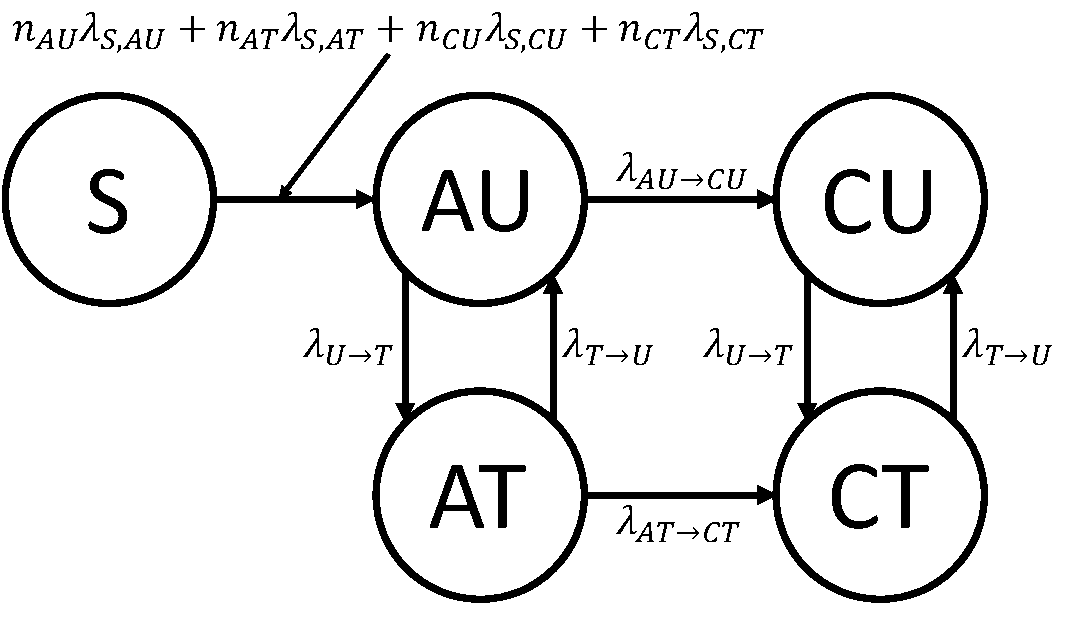
\includegraphics[width=0.75\textwidth]{figs/favites-model}
\caption[FAVITES Model]
{Epidemiological model of \gls{HIV} transmission with states Susceptible (S), Acute Untreated (AU), Acute Treated (AT), Chronic Untreated (CU), and Chronic Treated (CT). The model is parameterized by the rates of infectiousness of AU $(\lambda_{S,AU})$,  AT $(\lambda_{S,AT})$, CU $(\lambda_{S,CU})$, CT $(\lambda_{S,CT})$ individuals, and by the rate to transition from AU to CU $(\lambda_{AU \rightarrow CU})$, the rate to transition from AT to CT $(\lambda_{AT \rightarrow CT})$, the rate to start \gls{ART} $(\lambda_{U \rightarrow T})$, and the rate to stop ART $(\lambda_{T \rightarrow U})$.}
\label{fig:favites-model}
\end{figure}

We set $\lambda_{AU \rightarrow CU}$ such that the expected time to transition from AU to CU is 6 weeks~\cite{Bellan2015a} and set $\lambda_{AT \rightarrow CT}$ such that the expected time to transition from AT to CT is 12 weeks~\cite{Cohen2011}. We set $\lambda_{U \rightarrow T}$ such that the expected time to start ART is 1 year from initial infection~\cite{OBrien2012}, and we define \EART$=1/\lambda_{U \rightarrow T}$. We set $\lambda_{T \rightarrow U}$ such that the expected time to stop ART is 25 months from initial treatment~\cite{Nosyk2015}. For the rates of infection $\lambda_{S,j}$ for $j~\in~\{AU,CU,AT,CT\}$, using the infectiousness of CU individuals as a baseline, we set the parameters such that AU individuals are 5 times as infectious~\cite{Wawer2005} and CT individuals are not infectious (i.e., rate of 0). Cohen \textit{et al}. (2011) found a 0.04 hazard ratio when comparing linked \gls{HIV} transmissions between an early-therapy group and a late-therapy group~\cite{Cohen2011}, so we estimated AT individuals to be \sfrac{1}{20} the infectiousness of CU individuals. We then scaled these relative rates so that the total number of new cases over the span of the 10 years was roughly 6,000~\cite{Macchione2015}, yielding $\lambda_{S,AU}= 0.1125$.

\paragraph{Phylogeny.}  We estimate parameters related to phylogeny and sequences from real data. We used a \gls{MSA} of 674 HIV-1 subtype B \textit{pol} sequences from San Diego~\cite{Little2014} and a subset containing the 344 sequences that were obtained between 2005 and 2014. For both of these datasets, we inferred \gls{ML} phylogenetic trees using the ModelFinder Plus feature~\cite{Kalyaanamoorthy2017} of IQ-TREE~\cite{Chernomor2016}. We then removed outgroups from the tree inferred from the full 674 sequence dataset and used LSD~\cite{To2016} to estimate the \gls{tMRCA} and the per-year mutation rate distribution. The \gls{tMRCA} was estimated at 1980. The mutation rate was estimated as 0.0012 with a standard deviation of roughly 0.0003, so to match these properties, we sampled mutation rates for each branch independently from a truncated Normal random variable from 0 to infinity with a location parameter of 0.0008 and a scale parameter of 0.0005 to scale branch lengths from years to expected number of per-site mutations.

In our simulations, a single viral lineage from each individual was sampled at the end time of the epidemic (10 years). The viral phylogeny in unit of time (years) was then sampled under a coalescent model with logistic viral population growth using the same approach as the the PANGEA-HIV methods comparison exercise, setting the initial population to 1, the per-year growth rate to 2.851904, and the time back from present at which the population is at half the carrying capacity (\texttt{v.T50}) to -2~\cite{Ratmann2017}. Each seed individual is the root of an independent viral phylogenetic tree, and these trees were merged by simulating a seed tree with one leaf per seed node under a non-homogeneous Yule model~\cite{LeGat2016} scaled such that its height equals 25 years to match the 1980 estimate using SD. The rate function of the non-homogeneous Yule model was set to $\lambda(t)=e^{-t^2}+1$ to emulate short branches close to the base of the tree (see comparison to other functions in Fig.~\ref{fig:favites-seed-tree}).

\paragraph{Sequence data.} We sampled a root sequence from a profile \gls{HMM} generated from the San Diego \gls{MSA} using HMMER~\cite{Eddy1998}. We evolved it down the scaled viral phylogenetic tree under the \gls{GTR}+$\Gamma$ model using Seq-Gen~\cite{Rambaut1997} with parameters inferred by IQ-TREE (Table~\ref{tab:favites-params-evo}).

\paragraph{Varying parameters.} For San Diego, we explore four parameters (Table~\ref{tab:favites-params-main}). For the contact network, in addition to the \gls{BA} model, we used the \gls{ER}~\cite{Erdos1960} and \gls{WS}~\cite{Watts1998} models. We also varied the expected degree (\ED) of individuals in the contact network between 2 and 16 (Table~\ref{tab:favites-params-main}). For seed selection, we also used ``Edge-Weighted,'' where the probability that an individual is chosen is weighted by the individual's degree. For each selection of contact network model, \ED, and seed selection method, we study multiple rates of starting ART (expressed as \EART). In our discussions, we focus on \EART, a factor that the public health departments can try to impact. Increased effort in testing at-risk populations can decrease the diagnosis time, and the increased diagnosis rate coupled with high standards of care can lead to faster ART initiation. Behavioral intervention could in principle also impact degree distribution, another factor that we vary, but the extent of the effectiveness of behavioral interventions is unclear~\cite{Kelly1991}.

\begin{table}[!ht]
\caption[Simulation parameters]{Simulation parameters (base parameters in bold)}
\vspace{-0.25in}
\begin{center}
\begin{tabular}{|c|c|}
\hline
\textbf{Parameter} & \textbf{Values} \\
\hline
Contact Network Model & \textbf{\gls{BA}}, \gls{ER}, \gls{WS}\\
\hline
Expected Degree (\ED) & 2, \textbf{4}, 8, 16\\
\hline
Seed Selection & \textbf{Random}, Edge-Weighted\\
\hline
Mean Time to ART (\EART) & \sfrac{1}{8}, \sfrac{1}{4}, \sfrac{1}{2}, \textbf{1}, 2, 4, 8 (years)\\
\hline
\end{tabular}
\end{center}
\label{tab:favites-params-main}
\end{table}

\paragraph{Uganda simulations.} Our simulations with Uganda followed a similar approach to the base model used for San Diego but with different choices of parameters, motivated by Uganda. For inferring the reference phylogeny and mutation rates, we used a dataset of all 893 \gls{HIV}-1 subtype D \textit{pol} sequences in the \gls{LANL} \gls{HIV} Sequence Database that were sourced from Uganda and that were obtained between 2005 and 2014. All other Uganda parameters were motivated by McCreesh \textit{et al}. (2017)~\cite{McCreesh2017}, and the following are key differences from the San Diego simulation. The contact network had 10,000 total individuals (a regional epidemic), and 1,500 individuals were randomly selected to be seeds. For epidemiological parameters, we assumed the expected time to begin as well as stop ART to be 1 year~\cite{McCreesh2017}. A comprehensive list of simulation parameters can be found in Tables~\ref{tab:favites-params-epi}~and~\ref{tab:favites-params-evo}.

%% END FAVITES CHAPTER